\chapter{Exploratory Data Analysis}
\label{chapter_data_exploration}

As a preliminary step, we propose to perform an exploratory data analysis. This will give us some hints about the dataset, \eg the most important features, their correlation etc.

In order to have a first overview of the features, a short description is summarized in Table~\ref{tab_data_exploration}. It can be noticed the frequencies have low values, which makes sense since they are expressed in \si{\kilo\hertz}. 
The mean fundamental frequency is about \SI{143}{\hertz} which is coherent with the male and female fundamental frequencies~\cite{Traunmller1994}. 

Regarding the shape of the spectrum, the mean skewness indicates an average right-asymmetry of the spectrum. The mean kurtosis shows that the frequency distribution is leptokurtic. About the flatness of the spectrum, the features ``sfm'' and ``sp.ent'' seem to have inconsistent behaviour with respect to the their average value since one is above \num{0.5} and the other is below. However, the high standard deviation of ``sfm'' makes an analysis rather difficult.

%%%%%%%%%%%% TABLE %%%%%%%%%%%
\begin{table}[htb]
	\ra{1.2}
	\caption{Description of the features of the dataset}
	 \begin{subtable}{\textwidth}
			\centering
			\begin{tabular}{@{} c c c c  c c c c c c @{}}\toprule
				& meanfreq & sd & median & Q25 & Q75 & skew & kurt & sp.ent & sfm \\
			mean & \num{0.181} &\num{0.0571} & \num{0.186} & \num{0.140} & \num{0.225} & \num{3.14} &\num{36.6} & \num{0.895} &	\num{0.408} \\
			std & \num{0.0299} & \num{0.0167} & \num{0.0364} & \num{0.0487} & \num{0.0236} & \num{4.24} & \num{134} & \num{0.0450} & \num{0.178} \\
			min & \num{0.0394} & \num{0.0184} & \num{0.0110} & \num{0.000229} & \num{0.0429} & \num{0.142} & \num{2.07} & \num{0.739} & \num{0.0369} \\
			\SI{25}{\percent} & \num{0.164} & \num{0.0420} & \num{0.170} & \num{0.111} & \num{0.209} & \num{1.65} & \num{5.67} & \num{0.863} & \num{0.258} \\
			\SI{50}{\percent} & \num{0.185} & \num{0.0592} & \num{0.190} & \num{0.140} & \num{0.226} & \num{2.20} & \num{8.32} & \num{0.902} & \num{0.396} \\
			\SI{75}{\percent} & \num{0.199} & \num{0.0670} & \num{0.211}  & \num{0.176} & \num{0.244} & \num{2.93} & \num{13.7} & \num{0.929} & \num{0.534} \\
			max & \num{0.251} & \num{0.115} & \num{0.261} & \num{0.247} &
			\num{0.273} & \num{34.7} & \num{1310} & \num{0.982} & \num{0.843} \\ \bottomrule
			\end{tabular}
		\end{subtable}\hfill\null%

		\begin{subtable}{\textwidth}
			\centering
			\begin{tabular}{@{} c c c c  c c c c c @{}}\toprule
			 & mode & meanfun & minfun & maxfun & meandom & mindom & maxdom & modindx \\
			mean & \num{0.165} & \num{0.143} & \num{0.0368} & \num{0.259} & \num{0.829} & \num{0.0526} & \num{5.05} & \num{0.174} \\
			std & \num{0.0772} & \num{0.0323} & \num{0.0192} & \num{0.0301} & \num{0.525} & \num{0.0633} & \num{3.52} & \num{0.119} \\
			min & \num{0.00} & \num{0.0556} & \num{0.00977} & \num{0.103} & \num{0.00781} & \num{0.00488} & \num{0.00781} & \num{0.00} \\
			\SI{25}{\percent} & \num{0.118} & \num{0.117} & \num{0.0182} & \num{0.254} & \num{0.420} & \num{0.00781} & \num{2.07} & \num{0.0998} \\
			\SI{50}{\percent} & \num{0.187} & \num{0.140} & \num{0.0461} & \num{0.271} & \num{0.766} & \num{0.0234} & \num{4.99} & \num{0.139} \\
			\SI{75}{\percent} & \num{0.221} & \num{0.170} & \num{0.0479} & \num{0.277} & \num{1.18} & \num{0.0703} & \num{7.01} & \num{0.210} \\
			max & \num{0.280} & \num{0.238} & \num{0.204} & \num{0.279} & \num{2.96} & \num{0.459} & \num{21.87} & \num{0.932} \\ \bottomrule	
			\end{tabular}
		\end{subtable}\hfill\null%
	\label{tab_data_exploration}
\end{table}
%%%%%%%%%%%% END OF TABLE %%%%%%%%%%%

Regarding the distribution of the samples, there are \num{1584} recording of male voices and \num{1584} recording of female voices. So the classes are perfectly balanced.

Let us have a look to the correlation between the features. The correlation matrix, displayed in Figure~\ref{fig_corr_matrix}, exhibits high correlations between ``skew'' and ``kurt'' and between ``sp.ent'' and ``sfm'', which make sense since they quantify similar quantities. It can also be noticed that ``meanfreq'' and ``median'', ``Q25'', ``Q75'' are highly correlated which is self-evident given their definition. 
Thus, feature selection methods should be efficient in removing such redundancies in the dataset.
%%%%%%%%%%%% FIGURE %%%%%%%%%%%
\newlength{\BoxPlotFigWidth}
\newlength{\BoxPlotFigHeight}
\setlength{\BoxPlotFigWidth}{0.8\textwidth}
\settoheight{\BoxPlotFigHeight}{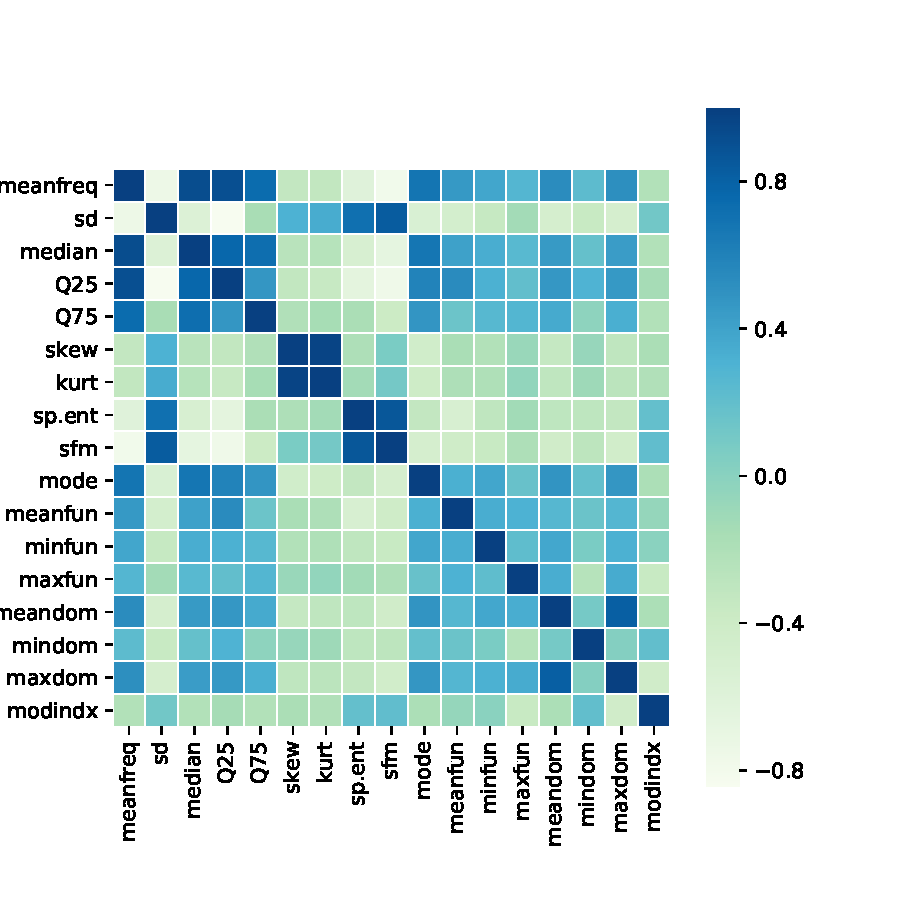
\includegraphics[width=\BoxPlotFigWidth]{figures/correlation_matrix.pdf}}
\begin{figure}[htb]
	\centering
	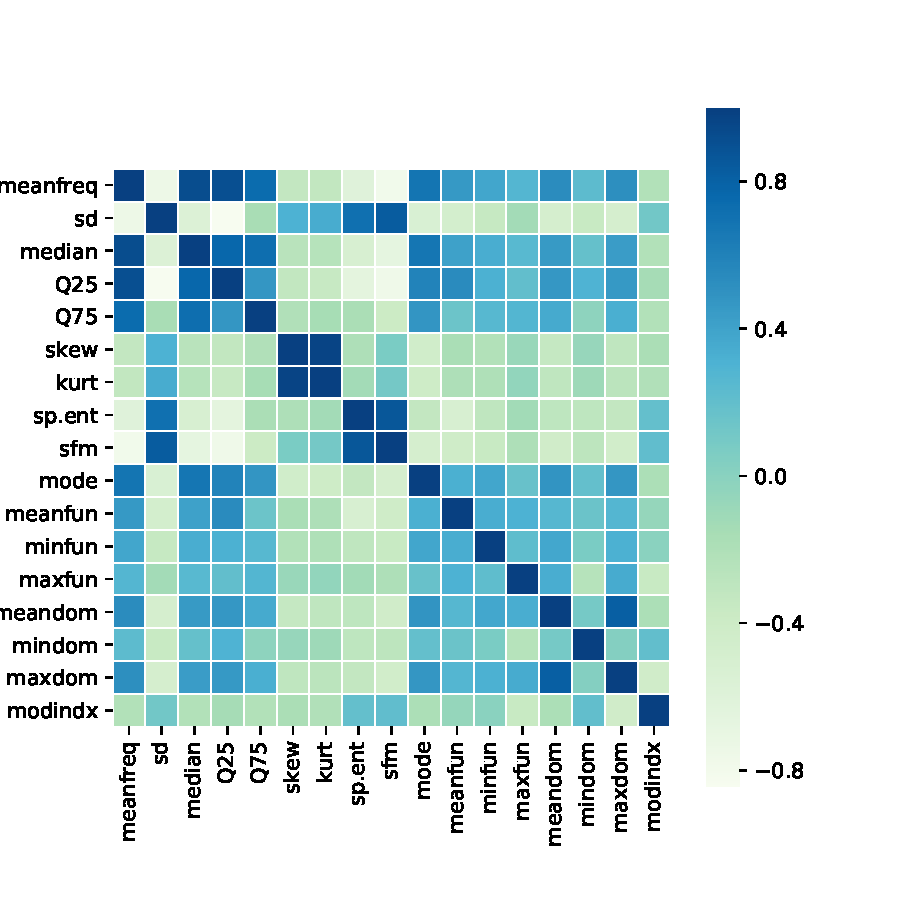
\includegraphics[height=\BoxPlotFigHeight]{figures/correlation_matrix.pdf}
	\caption{Correlation matrix of the dataset.}
	\label{fig_corr_matrix}
\end{figure}
%%%%%%%%%%%% END OF FIGURE %%%%%%%%%%%
%%%%%%%%%%%% FIGURE %%%%%%%%%%%
\setlength{\BoxPlotFigWidth}{0.48\textwidth}
\settoheight{\BoxPlotFigHeight}{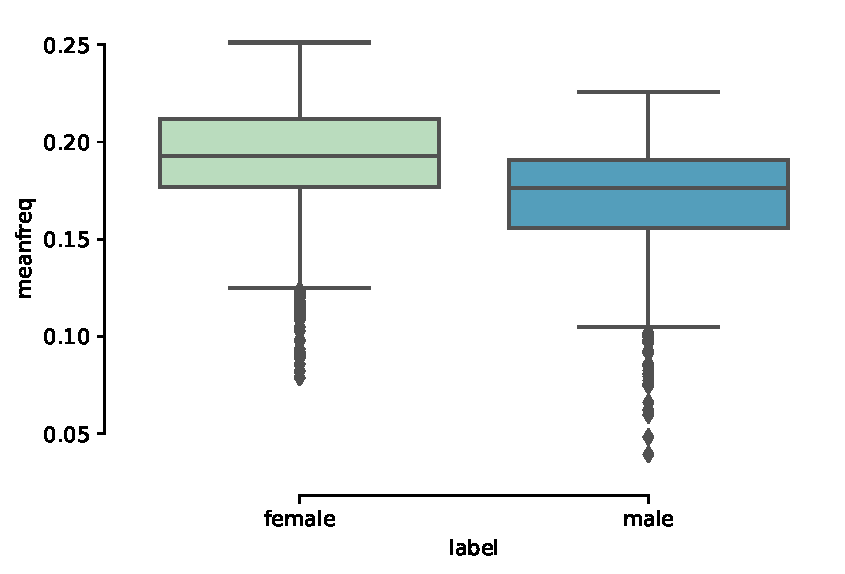
\includegraphics[width=\BoxPlotFigWidth]{figures/meanfreq_boxplot.pdf}}
\begin{figure}[htb]
	% Maximum length
	\hfill%
	\subcaptionbox{\label{fig_meanfreq_box}}{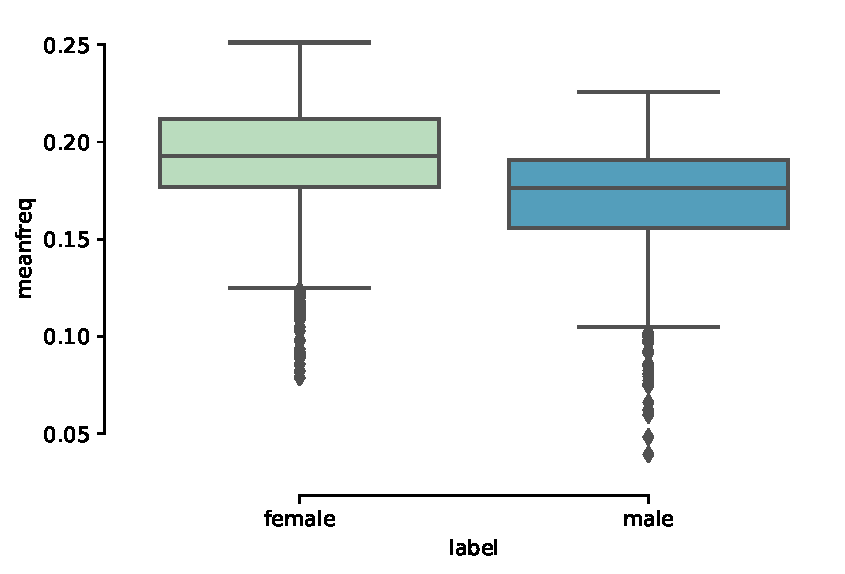
\includegraphics[height=\BoxPlotFigHeight]{figures/meanfreq_boxplot.pdf}}\hfill%
	\subcaptionbox{\label{fig_meanfun_box}}{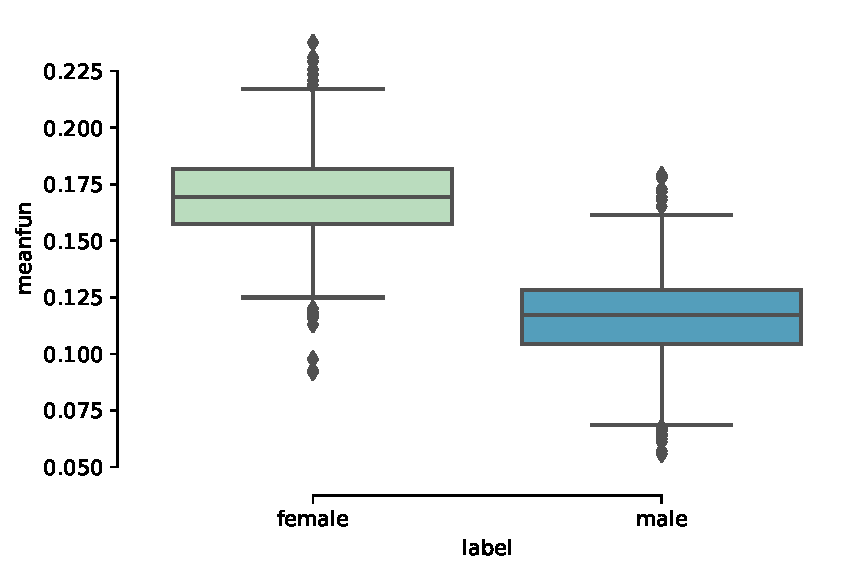
\includegraphics[height=\BoxPlotFigHeight]{figures/meanfun_boxplot.pdf}}\hfill\null%
	\caption{Box plots for (a)-``meanfreq'' and (b)-``meanfun'' features.}
	\label{fig_mean_freq}
\end{figure}
%%%%%%%%%%%% END OF FIGURE %%%%%%%%%%%

In the state-of-the-art, it appears that the fundamental frequency is a key feature for AGR, as stated in Chapter~\ref{chap:introduction}. Intuitively, we also think that the mean frequency should be a good classifier. In order to analyze this, Figs.~\ref{fig_meanfreq_box} and~\ref{fig_meanfun_box} represent the box plots of ``meanfreq'' and ``meanfun'' respectively. 
It can be noticed that ``meanfun'' is indeed a key feature for classification since the overlap between male and female is very low. Regarding ``meanfreq'', the overlap is bigger than for ``meanfun'' but remains rather low. 

Figs.~\ref{fig_meanfreq_facet} and~\ref{fig_meanfun_facet} represent the distribution of male and female with respect to ``meanfreq'' and ``meanfun'' respectively. They confirm the analysis made with the box plot, \ie{} that ``meanfun'' is a key component in AGR and is a far better classifier than ``meanfreq''.
%%%%%%%%%%%% FIGURE %%%%%%%%%%%
\settoheight{\BoxPlotFigHeight}{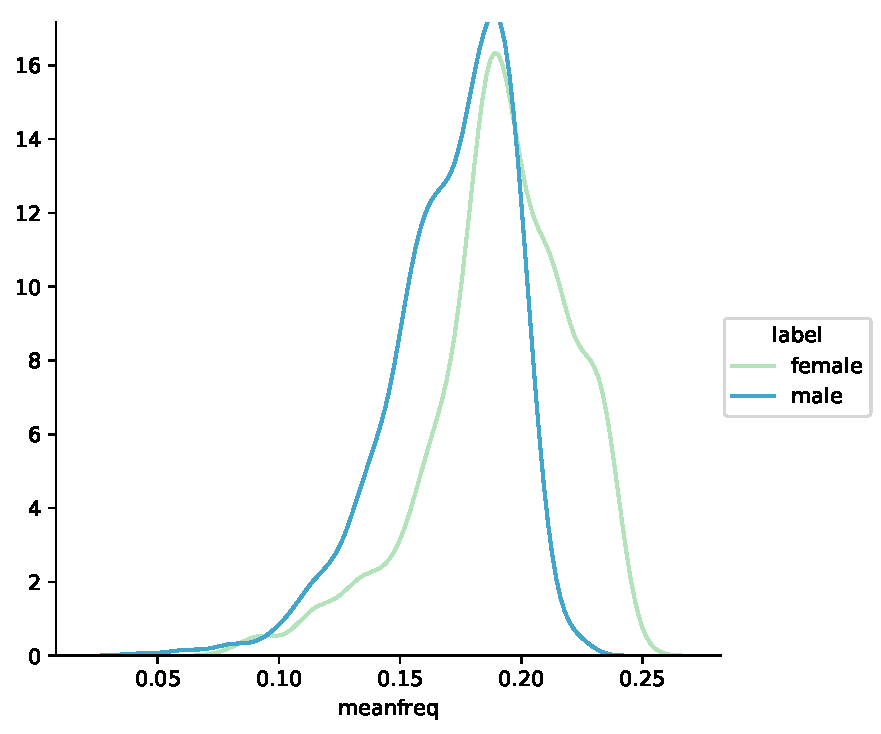
\includegraphics[width=\BoxPlotFigWidth]{figures/meanfreq_facetgrid.pdf}}
\begin{figure}[htb]
	% Maximum length
	\hfill%
	\subcaptionbox{\label{fig_meanfreq_facet}}{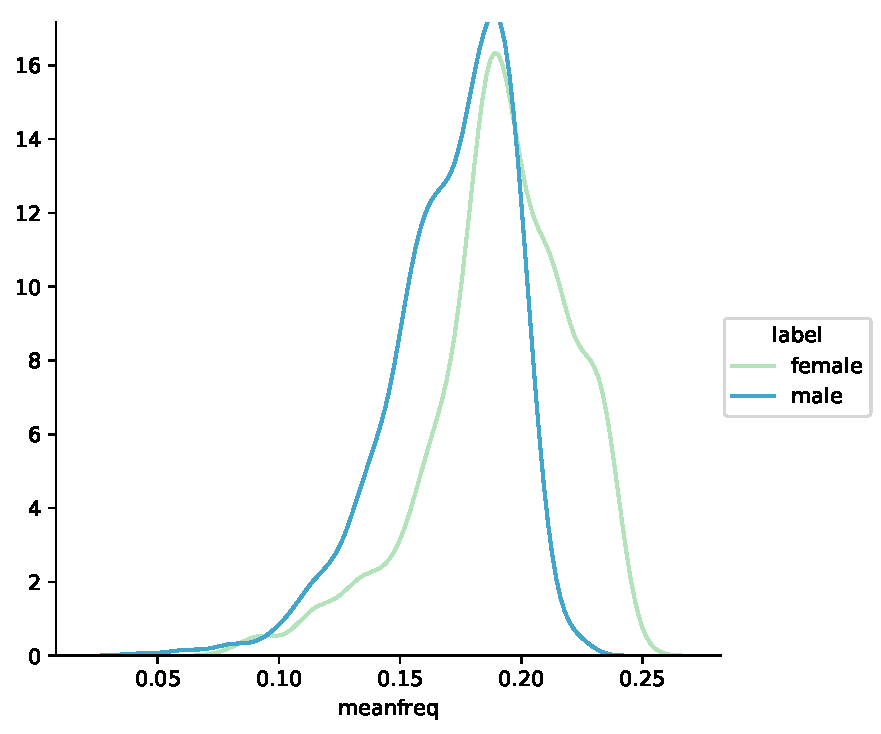
\includegraphics[height=\BoxPlotFigHeight]{figures/meanfreq_facetgrid.pdf}}\hfill%
	\subcaptionbox{\label{fig_meanfun_facet}}{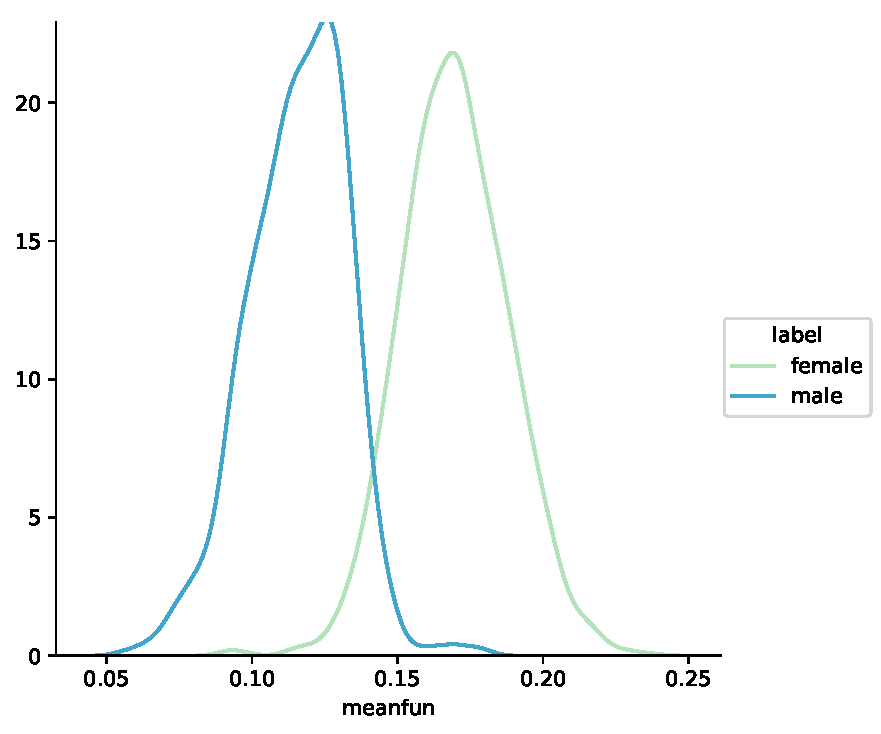
\includegraphics[height=\BoxPlotFigHeight]{figures/meanfun_facetgrid.pdf}}\hfill\null%
	\caption{Distribution of ``male'' and ``female'' for (a)-``meanfreq'' and (b)-``meanfun'' features.}
	\label{fig_facet}
\end{figure}
%%%%%%%%%%%% END OF FIGURE %%%%%%%%%%%

